% easychair.tex,v 3.1 2011/12/30
%
% Select appropriate paper format in your document class as
% instructed by your conference organizers. Only withtimes
% and notimes can be used in proceedings created by EasyChair
%
% The available formats are 'letterpaper' and 'a4paper' with
% the former being the default if omitted as in the example
% below.
%
\documentclass[procedia]{easychair}
%\documentclass[debug]{easychair}
%\documentclass[verbose]{easychair}
%\documentclass[notimes]{easychair}
%\documentclass[withtimes]{easychair}
%\documentclass[a4paper]{easychair}
%\documentclass[letterpaper]{easychair}

% This provides the \BibTeX macro
\usepackage{doc}
\usepackage{makeidx}
\usepackage[utf8]{inputenc}
\usepackage[T1]{fontenc}
\usepackage{amsmath}
\usepackage{amssymb}
\usepackage{subfig}


% In order to save space or manage large tables or figures in a
% landcape-like text, you can use the rotating and pdflscape
% packages. Uncomment the desired from the below.
%
% \usepackage{rotating}
% \usepackage{pdflscape}

% If you plan on including some algorithm specification, we recommend
% the below package. Read more details on the custom options of the
% package documentation.
%
% \usepackage{algorithm2e}

% Some of our commands for this guide.
%
\newcommand{\easychair}{\textsf{easychair}}
\newcommand{\miktex}{MiK{\TeX}}
\newcommand{\texniccenter}{{\TeX}nicCenter}
\newcommand{\makefile}{\texttt{Makefile}}
\newcommand{\latexeditor}{LEd}

\DeclareMathOperator*{\argmax}{arg\,max}
\DeclareMathOperator*{\argmin}{arg\,min}
\DeclareMathOperator{\sign}{sign}
\newtheorem{hypothesis}{Hypothesis}

\def\procediaConference{99th Conference on Topics of
  Superb Significance (COOL 2014)}

%\makeindex

%% Front Matter
%%
% Regular title as in the article class.
%
\title{Local Tuning in Peano Curves-based Global Optimization Scheme}

% \titlerunning{} has to be set to either the main title or its shorter
% version for the running heads. When processed by
% EasyChair, this command is mandatory: a document without \titlerunning
% will be rejected by EasyChair

\titlerunning{Local Tuning in Peano Curves-based \ldots}

% Authors are joined by \and. Their affiliations are given by \inst, which indexes into the list
% defined using \institute
%
\author{
    Vladislav V. Sovrasov%\thanks{Designed and implemented the class style}
}

% Institutes for affiliations are also joined by \and,
\institute{
  State University of Nizhny Novgorod,
  Nizhny Novgorod, Russia\\
  \email{sovrasov.vlad@gmail.com}
 }
%  \authorrunning{} has to be set for the shorter version of the authors' names;
% otherwise a warning will be rendered in the running heads. When processed by
% EasyChair, this command is mandatory: a document without \authorrunning
% will be rejected by EasyChair

\authorrunning{Sovrasov}

\begin{document}

\maketitle

\keywords{advanced numerical methods, deterministic global optimization, speedup of convergence, derivative-free algorithms}

\begin{abstract}
  In the present paper, one of the methods of accounting for the local information on
  the objective function in the Lipschitz global optimization problems has been considered.
  In the course of solving such problems, a problem of estimating Lipschitz constant of the
  objective function arises. According to the classic scheme, such an estimate is a single one
  for the whole search domain. The method of accounting for the local properties is based on
  the building of the estimates of Lipschitz constants for the search subdomains and has been
  investigated earlier for the one-dimensional case. For solving the multidimensional problems,
  the dimension reduction is applied. A multidimensional optimization problem is reduced to
  a one-dimensional problem, which the objective function satisfy Hölder condition in.
  In this paper, the application of building the local estimates of Hölder constant in the
  reduced multidimensional optimization problems using the same scheme to the one used
  in the one-dimensional Lipschitzian problems is considered.
\end{abstract}

%\setcounter{tocdepth}{2}
%{\small
%\tableofcontents}

%\section{To mention}
%
%Processing in EasyChair - number of pages.
%
%Examples of how EasyChair processes papers. Caveats (replacement of EC
%class, errors).


%------------------------------------------------------------------------------
\section{Introduction}
\label{sect:introduction}

The one-dimensional characteristical algorithms represent one of the classes of the
optimization algorithms used widely \cite{optHandbook}. A number of schemes of reduction of the
multidimensional problems to one or several one-dimensional ones, i. e. the \textit{dimension
reduction} schemes have been developed \cite{evolvents2013}, \cite{gergelGrishaginStringin2013}.
All these schemes can be efficiently parallelized \cite{optParallelBook}.
\par
In recent years, when building the global optimization algorithms, an increased attention
is paid to accounting for the local properties of the objective function. In the
case of the characteristical schemes, this approach allows developing a mixed algorithm
\cite{mixedAlg} as well as using different estimates of Lipschitz constant in different search
domain \cite{sergLocalTuningFirst}. Originally, the latter approach has been proposed for the one-dimensional
problems, also the investigation of this one when using the nested optimization scheme
has been carried out \cite{nestedLocal}. In all these cases, this approach have demonstrated itself to
be an efficient one, having allowed accelerating the convergence of the
optimization methods essentially. In the present paper, a generalization of the method
for building of the local estimates of Lipschitz constants onto the case of Hölder
functions obtained when reducing the multidimensional optimization problems is considered.

%------------------------------------------------------------------------------
\section{Problem Statement}
\label{sect:problem}

The global optimization problem can be formulated as follows:
to find the global minimum of an \(N\)-dimensional function \(\varphi(y)\) in a hyperinterval
\(D=\{y\in R^N:a_i\leqslant x_i\leqslant{b_i}, 1\leqslant{i}\leqslant{N}\}\): \(\varphi(y^*)=\min\{\varphi(y):y\in D\}\).
In order to obtain an estimate of the global minimum from a finite number of computations
of the function values, \(\varphi(y)\) is required to satisfy Lipschitz condition.
\begin{displaymath}
\label{lip}
|\varphi(y_1)-\varphi(y_2)|\leqslant L\Vert y_1-y_2\Vert,y_1,y_2\in D,0<L<\infty
\end{displaymath}
\par
The use of the evolvents \(y(x)\) i. e. the curves filling the space is a classic scheme
for the dimension reduction for the global optimization algorithms \cite{strOptBook}.
\begin{displaymath}
\label{cube}
\lbrace y\in R^N:-2^{-1}\leqslant y_i\leqslant 2^{-1},1\leqslant i\leqslant N\rbrace=\{y(x):0\leqslant x\leqslant 1\}
\end{displaymath}
\par
Such a mapping allows reducing a problem stated in a multidimensional space to solving
a one-dimensional one at the expense of worsening its properties. In particular,
the one-dimensional function \(\varphi(y(x))\) is not a Lipschitz one but is a Hölder one:
\begin{displaymath}
\label{holder}
|\varphi(y(x_1))-\varphi(y(x_2))|\leqslant H{|x_1-x_2|}^{\frac{1}{N}},x_1,x_2\in[0,1]
\end{displaymath}
where Hölder constant \(H\) is related to Lipschitz constant \(L\) by the relation
\begin{displaymath}
H=4Ld\sqrt{N},d=\max\{b_i-a_i:1\leqslant i\leqslant N\}
\end{displaymath}
\par
Therefore, not limiting the generality, one can consider the minimization of the
one-dimensional function \(f(x)=\varphi(y(x))\), \(x\in[0;1]\) satisfying Hölder condition.
The issues of numerical building of the mapping like Peano curve and the corresponding
theory have been considered in details in \cite{strOptBook}. Here we would note that an evolvent
built numerically is an approximation to the theoretical Peano curve with the precision
of the order \(2^{-m}\) where \(m\) is the building parameter of the evolvent.

%------------------------------------------------------------------------------
\section{Description of the Algorithm}
\label{sect:algorithm}

The considered algorithm of solving the stated problem implies the building of
a sequence of points \(x_k\), which the values of the minimized function \(z_k = f(x_k)\)
are computed in. Let us call the process of computation of the function value
(including the building of an image \(y_k=y(x_k)\)) a trial, and the pair \((x_k,z_k)\) ---
the result of the trial. A set of the pairs \(\{(x_k,z_k)\}, 1\leqslant k\leqslant n\)
makes the search information accumulated by the method after executing \(n\) steps.
\par
At the first iteration of the method, a trial is executed in an arbitrary internal
point \(x_1\) of the interval \([0,1]\). Let us assume \(n \geqslant 1\) iterations
of the method to be completed, in the course of which the iterations in \(k = k(n)\)
points \(x_i, 1\leqslant i\leqslant k\) have been performed. Then, the point \(x^{k+1}\)
of the search trial of the next \((k+1)\)th iteration is determined in accordance with the rules:
\par
Step 1. Renumber the points of the set \(X_k=\{x^1,\dotsc,x^k\}\cup\{0\}\cup\{1\}\),
which includes the boundary points of the interval \([0,1]\) as well as the points of
preceding trials, by the lower indices in the order of increasing the values of coordinate i. e.
\begin{displaymath}
0=x_0<x_1<\dotsc<x_{k+1}=1
\end{displaymath}
\par
Step 2. Assuming \(z_i=f(x_i),1\leqslant i\leqslant k\), compute the quantities
\begin{equation}
\label{step2}
\mu=\max_{1\leqslant i\leqslant k}\dfrac{|z_i-z_{i-1}|}{\Delta_i},
\begin{matrix}
    M =
    \left\{
    \begin{matrix}
    r\mu,\mu>0 \\
    1,\mu=0
    \end{matrix} \right.
    \end{matrix}
\end{equation}
where \(r\) is a predefined parameter of the method, and \(\Delta_i=(x_i-x_{i-1})^\frac{1}{N}\).
\par
Step 3. For each interval \((x_{i-1},x_i),1\leqslant i\leqslant k+1\), compute the
characteristics according to the formulae
\begin{equation}
\label{step3_1}
R(1)=2\Delta_1-4\dfrac{z_1}{M},R(k+1)=2\Delta_{k+1}-4\dfrac{z_k}{M}
\end{equation}
\begin{equation}
\label{step3_2}
R(i)=\Delta_i+\dfrac{(z_i-z_{i-1})^2}{M^2\Delta_i}-2\dfrac{z_i+z_{i-1}}{M},1<i<k+1
\end{equation}
\par
Step 4. Select the interval \((x_{t-1}, x_t)\) such that
\begin{equation}
\label{step4}
t=\argmax_{1\leqslant i \leqslant k+1}R(i),
\end{equation}
i.e., the interval with the maximal characteristic.
\par
Step 5. Execute new trial in the point \(x_{k+1}\) computed according to the formulae
\begin{displaymath}
x_{k+1}=\dfrac{x_{t}+x_{t-1}}{2},t=1,t=k+1
\end{displaymath}
\begin{equation}
\label{step5}
x_{k+1}=\dfrac{x_{t}+x_{t-1}}{2}-\sign(z_{t}-z_{t-1})\dfrac{1}{2r}\left[\dfrac{|z_{t}-z_{t-1}|}{\mu}\right]^N,1<t<k+1
\end{equation}
\par
The algorithm is terminated if the condition \(\Delta_{t}\leqslant \varepsilon\) is fulfilled;
here \(\varepsilon>0\) is a predefined precision. As an estimate of the global optimum solution of the problem the values
\begin{equation}
f_k^*=\min_{1\leqslant i \leqslant k}f(x_i), x_k^*=\argmin_{1\leqslant i \leqslant k}f(x_i)
\end{equation}
are selected. The theoretical substantiation of this method is presented in \cite{strOptBook}.

%------------------------------------------------------------------------------
\section{Local Adaptive Estimate of Hölder Constant}
%\label{sect:algorithm}
At it is seen from the scheme of the algorithm, regardless to the local properties
of the optimized one-dimensional function, the same values of estimate of Hölder
constant (\ref{step2}) is used to compute the characteristic of all intervals (\ref{step3_1}), (\ref{step3_2}).
In \cite{sergLocalTuning}, it has been proposed to use different values of \(M\) for each interval,
and also the efficiency of this approach in the case of the optimization of the
one-dimensional functions satisfying Lipschitz condition has been shown. In \cite{nestedLocal},
the application of the adaptive estimates of Lipschitz constants in the multidimensional
nested optimization scheme has been considered. For each interval, the local estimate of the
constant is an additive convolution of the ``global'' and ``local'' ones (\(\gamma\) and \(\lambda\), correspondingly):
\begin{displaymath}
  \begin{array}{lr}
    \lambda_i=\max\{H_{i-1},H_i,H_{i+1}\} \\
    H_i=\frac{|z_i-z_{i-1}|}{\Delta_i} \\
    H^k=\max\{H_i:i=2,\dots ,k\} \\
    \gamma_i=H^k\frac{\Delta_i}{\Delta^{max}} \\
    \Delta^{max}=\max\{\Delta_{i}:i=2,\dots ,k\}
  \end{array}
\end{displaymath}
\begin{equation}
\label{additiveConv}
M_i=r\cdot \max\{H_i, \frac{1}{2}(\lambda_i+\gamma_i),\xi\}
\end{equation}
\(\xi\) is chosen small to prevent the case of the function being constant over search interval.
This variant of convolution does not depend on the parameter \(r\), however, the adaptive convolution:
\begin{equation}
\label{additiveAdaptiveConv}
M_i=r\cdot \max\{H_i, \frac{\lambda_i}{r}+\frac{r-1}{r}\gamma_i,\xi\}
\end{equation}
has been considered in \cite{sergLocalTuning} as well.
If it is known a priori that the optimized function has a complex shape with multiple
local minima, then the initial value of \(r\) is specified to be large enough that
results in the dominance of the ``global'' component \(\gamma\) in the adaptive convolution.

%------------------------------------------------------------------------------
\section{Hypothesis about Convergence}
%\label{sect:algorithm}
In \cite{sergLocalTuning}, a theorem on the convergence of the method in the case if the objective
function is Lipschitz one is given. However, as a rule, such statements are true in
Hölder metrics as well, therefore, presumably, the following hypothesis is true:

\begin{hypothesis}
Assume the objective function \(f(x)\) to  satisfy Hölder condition with finite
constant \(H > 0\), and let x be a limit point of \(\{x_k\}\) generated by the algorithm.
Then, the following assertions hold:
\begin{enumerate}
  \item If \(x\in(0;1)\), then convergence to \(x\) is a bilateral one i. e. there
  exist two infinite subsequences of \(\{x_k\}\) converging to \(x\): one from the
  left, the other from the right;
  \item \(f(x_k) \geqslant f(x)\) for all trial points \(x_k, k \geqslant 1\);
  \item If there exists another limit point \(x^* = x\), then \(f(x) = f(x^*)\);
  \item If the function \(f(x)\) has a finite number of local minima in \([0, 1]\),
  then the point \(x\) is a local optimum one;
  \item (Sufficient conditions for convergence to a global minimizer). Let \(x^*\)
  be a global minimizer of \(f(x)\). If there exists an iteration number \(k^*\)
  such that for all \(k > k^*\) the inequality
  \(M_j(k) > H_j(k)\) holds, where \(H_j(k)\) is Hölder constant for the interval
  \([x_{j(k)-1}, x_{j(k)}]\) containing \(x^*\), and \(M_{j(k)}\) is its estimate.
  Then, the set of limit points of the sequence \(\{x_k\}\) coincides with the set
  of global minimizers of the function \(f(x)\).
\end{enumerate}
\end{hypothesis}

The proof of this hypothesis requires further theoretical studies. Within the frames of
the present work, it is not performed. The convergence has been established numerically only.

%------------------------------------------------------------------------------
\section{Results of Experiments}
\label{sect:experiments}

The experiments on the evaluation of the efficiency of the method with the local
adaptive estimate of Hölder constant have been carried out using the two-dimensional
classes of Grishagin problems (\(F_{GR}\)) \cite{grishaginClass} and GKLS ones \cite{gklsClass}. Each class
includes 100 multiextremal functions. In all experiments, the evolvent was built
with the density \(m = 12\), parameter \(\varepsilon\) in the termination criterion was equal \(10^{-3}\).
The parameter \(r\) was selected as low as possible, allowing to solve all the
problems. The search step for \(r\) was \(0.1\).
\par
For clarity of illustration of the advantages of the local adaptive scheme of estimating
the constant \(H\), let us consider a particular example of the results obtained by the method.
In Fig. \ref{fig:grish_isolines}, the level lines of a function from \(F_{GR}\) class and the trial
points executed by the method with the global estimate of Hölder constant and with
the one estimated according to formula (\ref{additiveConv}) are shown. As it is
seen from the figures, the method with global estimate of the constant executes a
large number of trials in the nearness of the global minimizer (total 1086 trials
have been executed) before the termination condition is satisfied, whereas the method
with the local adaptive estimate converges much faster (total 385 trials have been executed).
The same situation takes place when optimizing a function from GKLS class (Fig. \ref{fig:gkls_isolines}).
The method with the global estimate of the constant had executed 2600 trials while
the method with the local adaptive estimate had executed 1190 trials only.
\begin{figure}[ht]
    \centering
    \subfloat[global \(H\) estimation]{{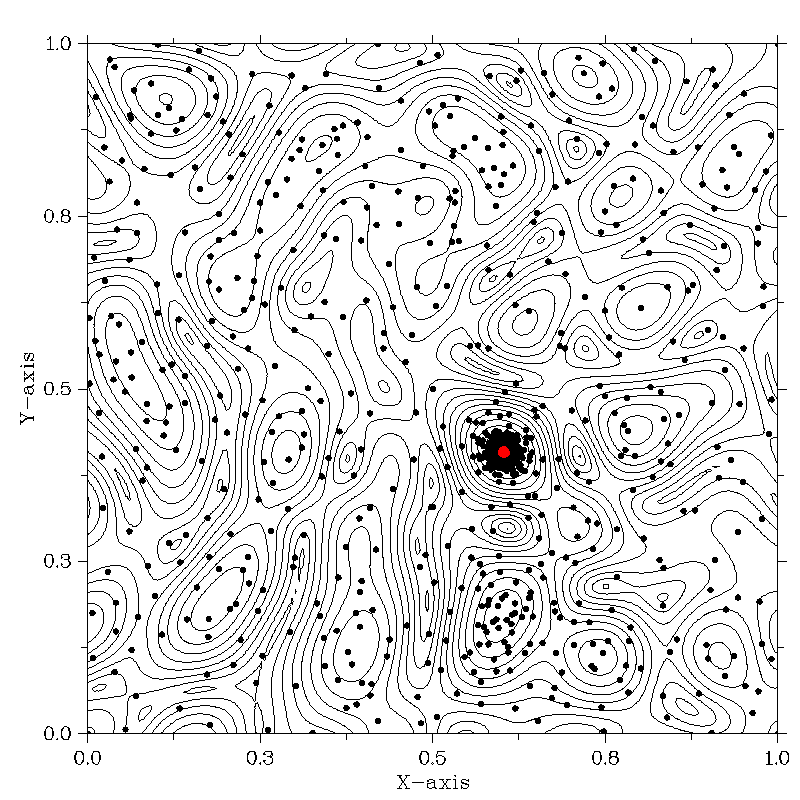
\includegraphics[width=0.45\textwidth]{images/gs_glob.png} }}
    \qquad
    \subfloat[local-adaptive \(H\) estimation]{{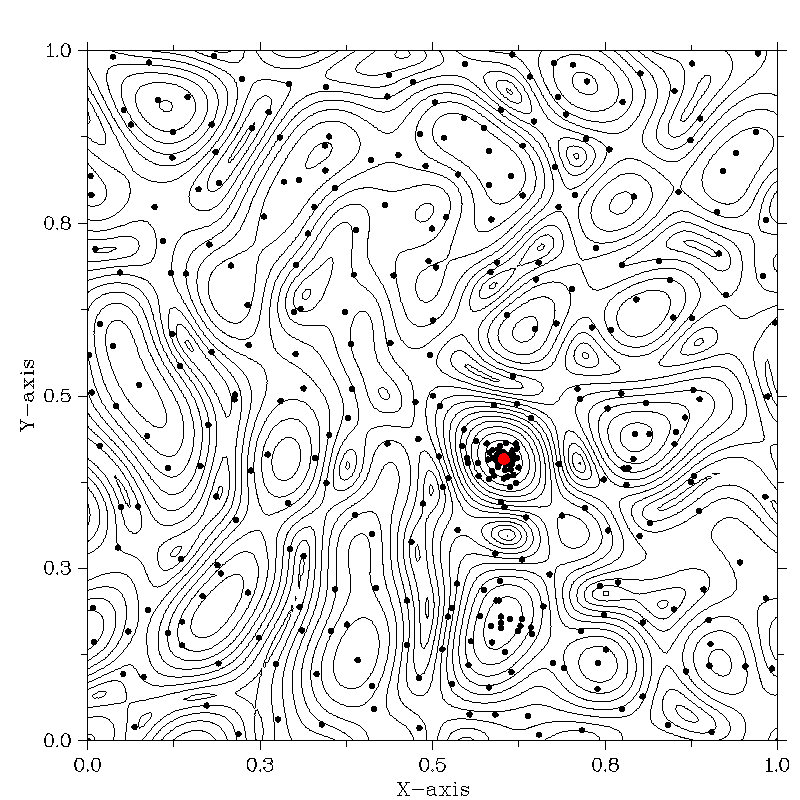
\includegraphics[width=0.45\textwidth]{images/gs_loc.png} }}
    \caption{The level lines of a function from \(F_{GR}\) class}
    \label{fig:grish_isolines}
\end{figure}

\begin{figure}[ht]
    \centering
    \subfloat[global \(H\) estimation]{{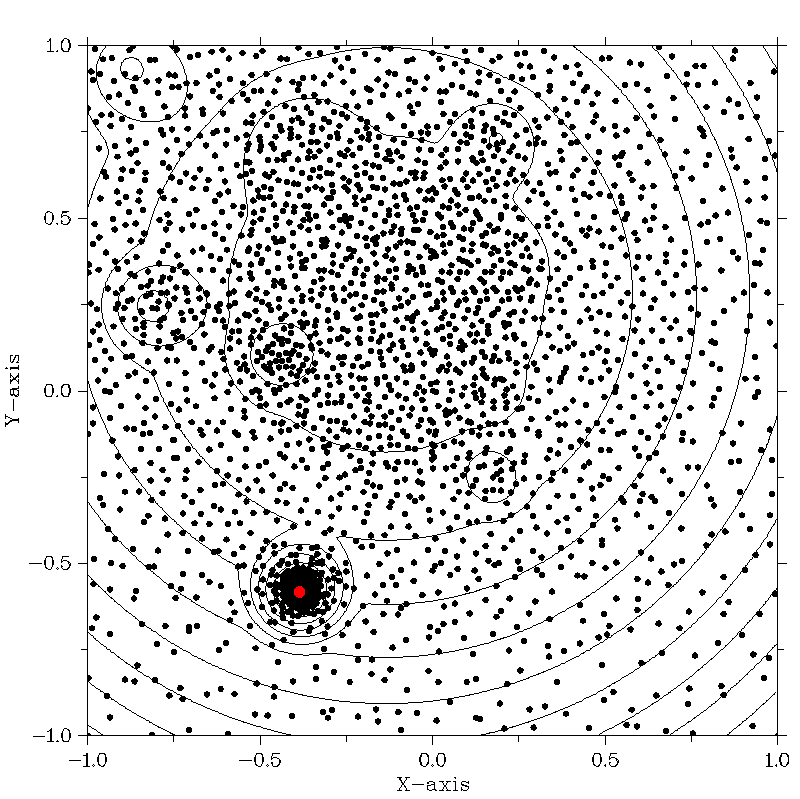
\includegraphics[width=0.45\textwidth]{images/gkls_glob.png} }}
    \qquad
    \subfloat[local-adaptive \(H\) estimation]{{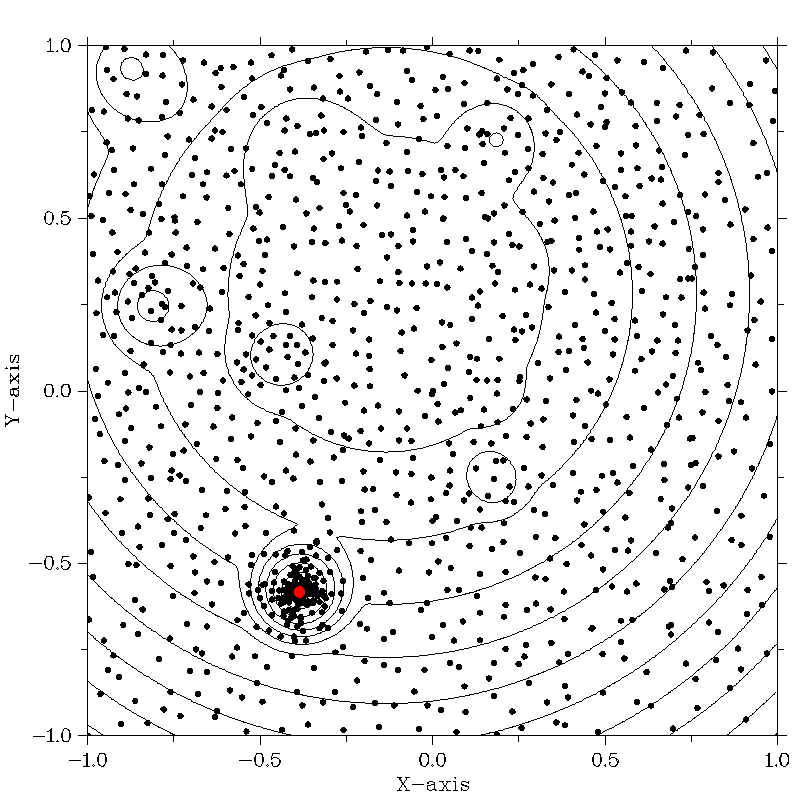
\includegraphics[width=0.45\textwidth]{images/gkls_loc.png} }}
    \caption{The contour plots of a function from GKLS class}
    \label{fig:gkls_isolines}
\end{figure}
\par
Next, let us go to the comparison of various variants of the method for the problem
classes considered. In order to evaluate the efficiency of an algorithm, we will use
the operating characteristics \cite{grishaginClass}, which is defined by a set of points on the \((K, P)\)
plane where \(K\) is the averaged number of the search trials carried out before the satisfaction
of the termination condition when minimizing a function from given class, and \(P\)
is portion of problems solved successfully. If at given \(K\) the operating characteristic
of a method goes higher than the one of another method, it means that at fixed costs
of the search the former method will find the solution with a greater probability.
If some value of \(P\) is fixed, and the characteristic of a method goes to the left from
the one of another method, the former method requires fewer resources to achieve the same reliability.
\par
\begin{figure}[ht]
  	\center
    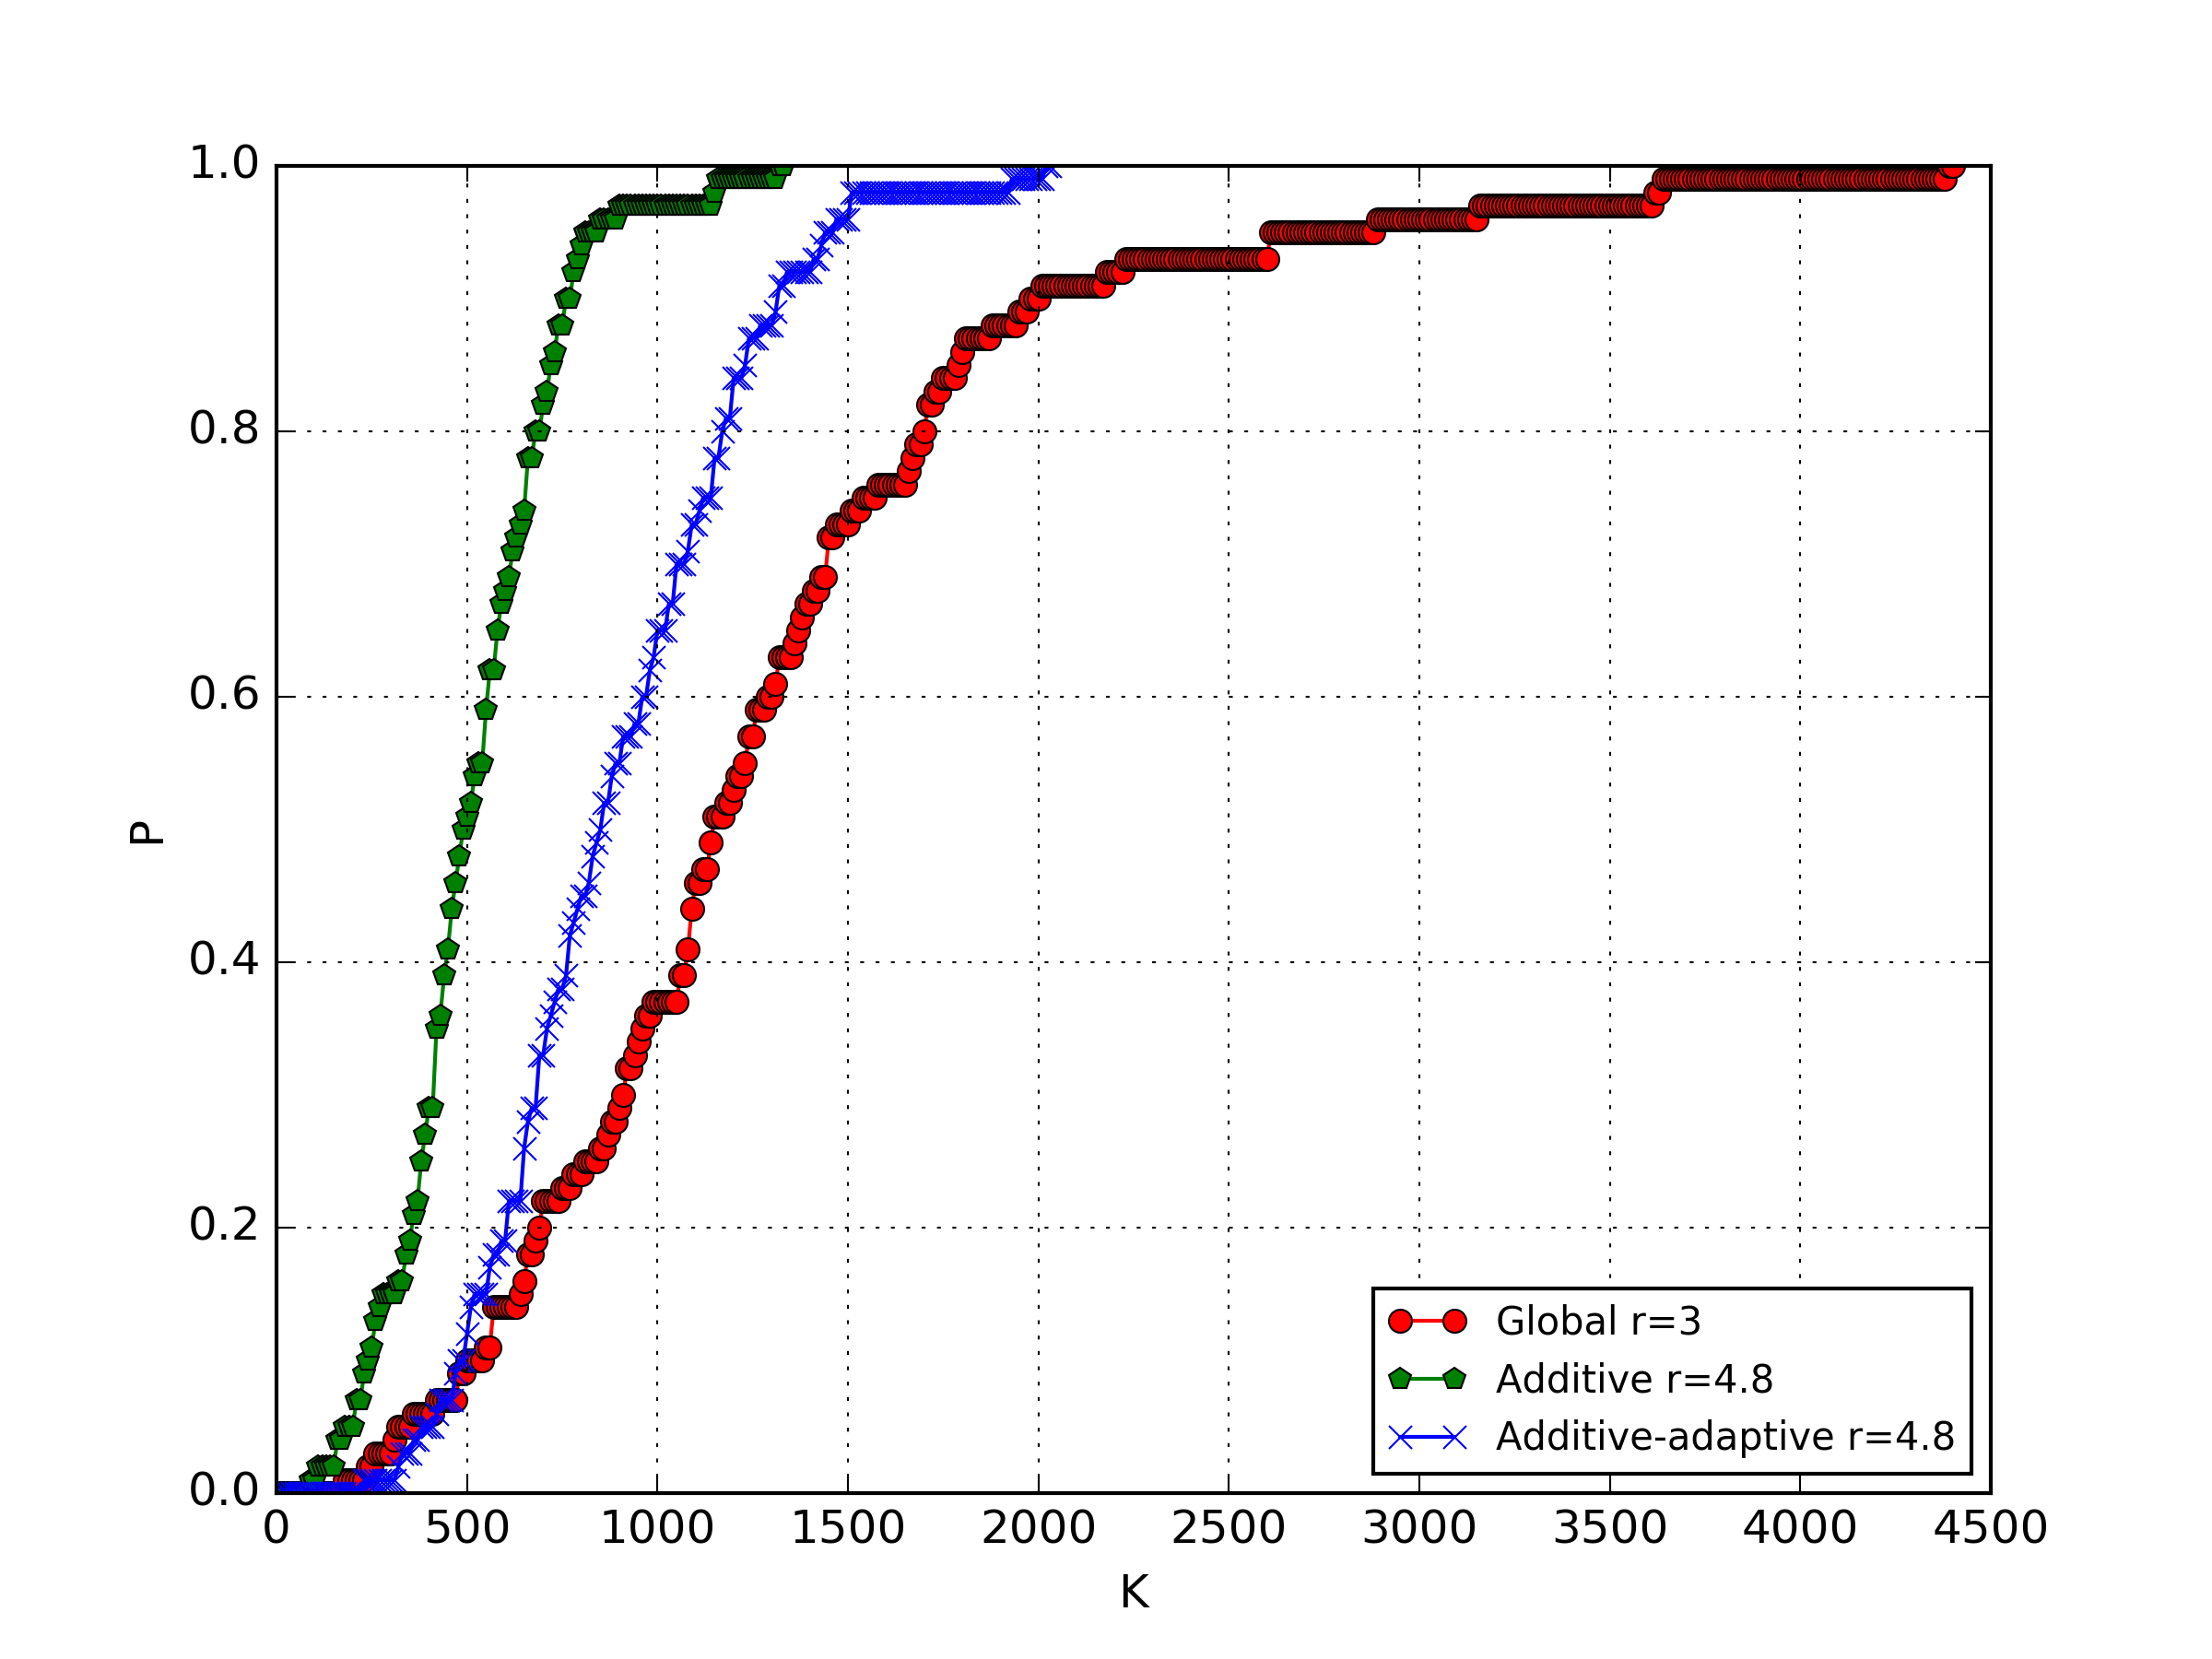
\includegraphics[width=0.75\textwidth]{images/grishagin.png}
    \caption{Operating characteristics of the methods compared on \(F_{GR}\) problems class}
    \label{fig:grishh_op}
  \end{figure}
As it is seen from the operating characteristics in Fig. \ref{fig:grishh_op}, \ref{fig:gkls_op}, both methods with the
local adaptive estimate of Hölder constant have demonstrated an essential advantage.
However, both methods require setting a higher value of the parameter \(r\). If one compares the
methods with the adaptive convolution and  with the non-adaptive one (\ref{additiveConv})(\ref{additiveAdaptiveConv}), the advantage
of the latter is seen clearly, although it requires a higher value of the reliability
parameter \(r\) to solve the problems form GKLS class.
  \begin{figure}[ht]
  	\center
    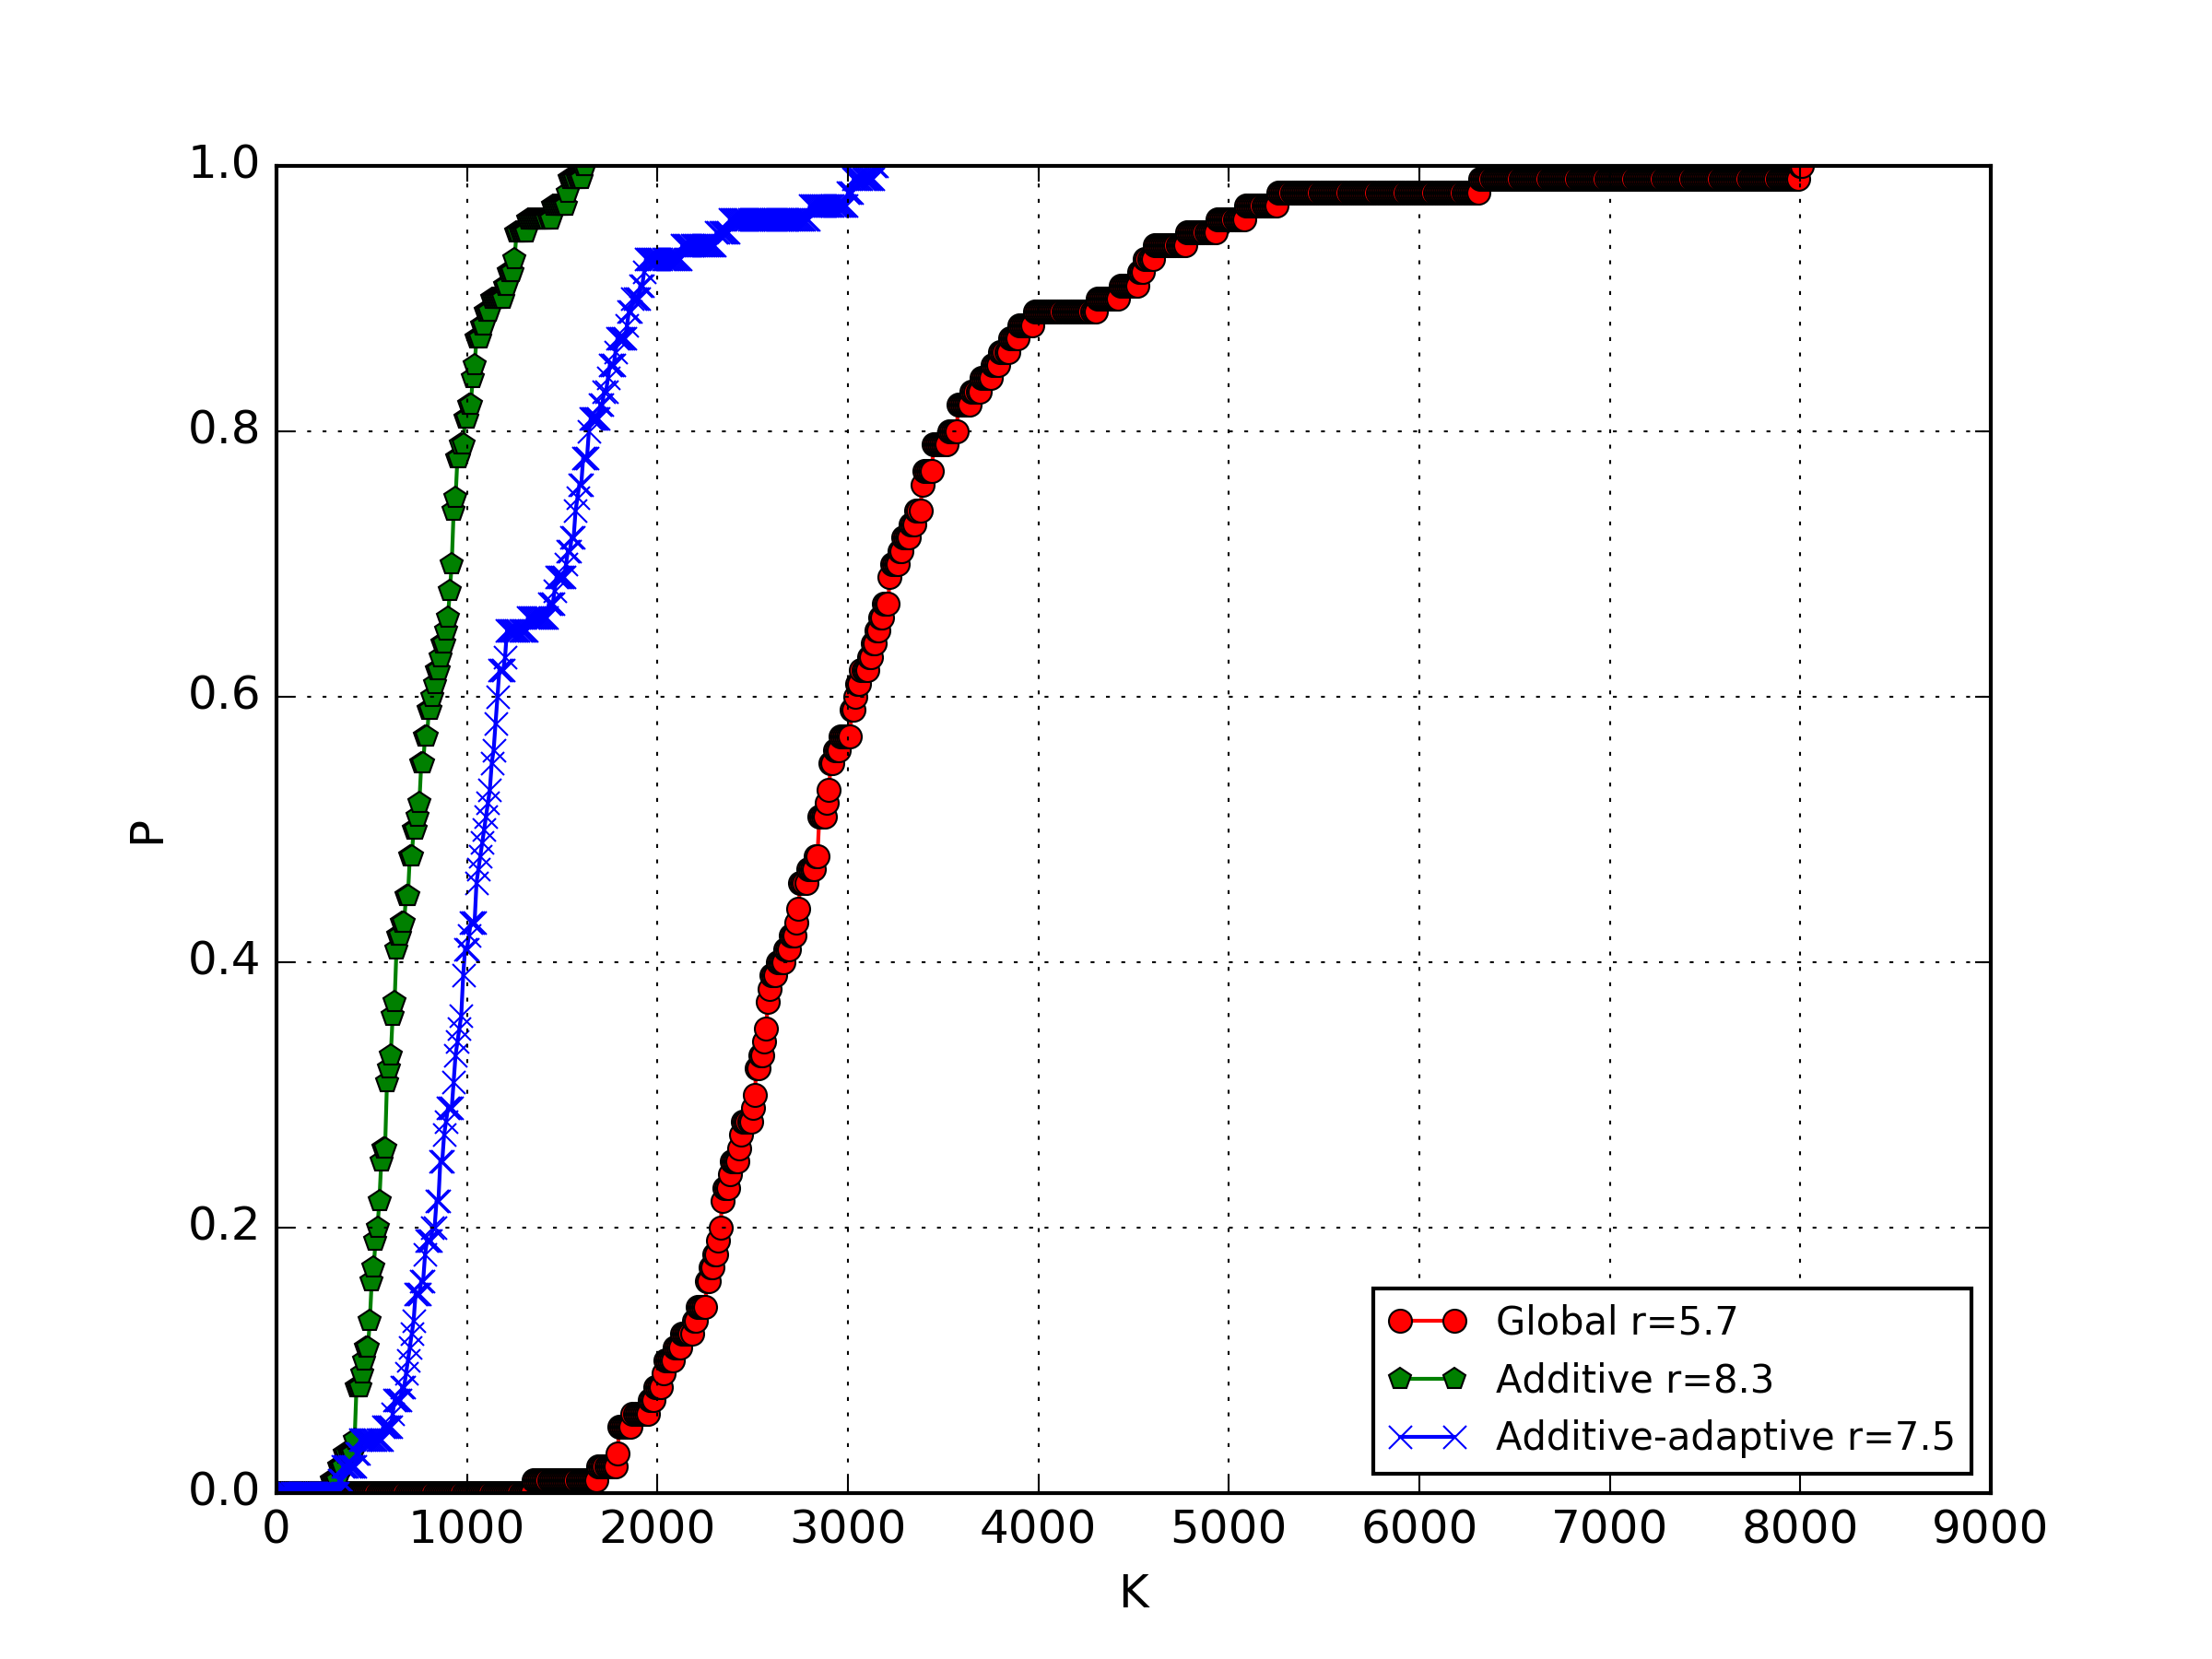
\includegraphics[width=0.75\textwidth]{images/gkls-s.png}
    \caption{Operating characteristics of the methods compared on GKLS problems class}
    \label{fig:gkls_op}
  \end{figure}
%------------------------------------------------------------------------------
\section{Conclusions}
In the present work, the global optimization problems and the deterministic methods
for solving these ones are considered. The relevance of solving the problems of this
class is defined by the importance of the applications (optimal design, problems of
parameter identification, pattern recognition, signa processing, etc.). The multiextremal
(global) optimization methods are extremely computation costly since these ones require
the constructing and using of the adaptive models of the objective function behavior
according to the trial results accumulated during the algorithm execution.
\par
In this work, the application of the method of accounting for the local behavior of
the optimized function within the multidimensional multiextremal optimization method
has been considered. Earlier, this method has been applied to the one-dimensional
problems only. Taking into account the local properties is implemented in the use of
different estimates of Hölder constant in different search domains. Thus, the process
of solving the problem is accelerated significantly by means of reducing the number of
the search trials.
\par
The comparison of two different schemes of constructing the estimates of Hölder constant
(\ref{additiveConv}), (\ref{additiveAdaptiveConv}) has revealed the advantage of scheme (\ref{additiveConv}).
However, a larger value of the reliability parameter of the search method \(r\) might be required
to use this scheme for solving some problems. When solving the complex problems with a small
area of attraction of the global extremum, scheme (\ref{additiveAdaptiveConv}) is preferable for
more reliability of the method. The efficiency of the considered approach has been confirmed
by solving the series of multidimensional problems form two classes.

%------------------------------------------------------------------------------
\section{Acknowledgements}
This research was supported by the Russian Science Foundation, project No 16-11-10150
``Novel efficient methods and software tools for the time consuming decision making problems
with using supercomputers of superior performance''.

%------------------------------------------------------------------------------
% Refs:
%
\label{sect:bib}
%\bibliographystyle{plain}
%\bibliographystyle{alpha}
\bibliographystyle{unsrt}
%\bibliographystyle{abbrv}
\bibliography{ysc_paper}

%------------------------------------------------------------------------------
% Index
%\printindex

%------------------------------------------------------------------------------
\end{document}

% EOF
